\documentclass[11pt]{beamer}

\usetheme{Madrid}
\usecolortheme{default}

% --- Load leopard.sty from parent directory ---
% TEXINPUTS should include the paper directory or we copy leopard.sty
\usepackage{leopard}
\renewcommand{\mathrm}[1]{\mathsf{#1}}

% --- Project-specific overrides for slides ---
\renewcommand{\phi}{\varphi}
\newcommand{\Rep}{\mathrm{Rep}}
\newcommand{\mqty}[1]{\begin{bmatrix*}[r]#1\end{bmatrix*}}

\newcommand{\pwplus}{\mathbin{\dot{+}}}
\newcommand{\pwminus}{\mathbin{\dot{-}}}
\newcommand{\pwcdot}{\mathbin{\dot{\cdot}}}
\newcommand{\pwtimes}{\mathbin{\dot{\times}}}
\newcommand{\pwzero}{\mathbin{\dot{0}}}
\newcommand{\pwone}{\mathbin{\dot{1}}}

% --- Beamer customization ---
\setbeamertemplate{navigation symbols}{}
\setbeamertemplate{footline}[frame number]

\title{Representations of Lie Groups\\A Mathematical Dissection of Quantum Spin}
\subtitle{Part I: Mathematical Foundations}
\author{Gordon Chan\\Supervisor: Assoc. Prof. François Gay-Balmaz}
\date{28 July 2026}

\begin{document}

% ======================================================================
\frame{\titlepage}

% ======================================================================
\begin{frame}{Roadmap}
\tableofcontents
\end{frame}

% ======================================================================
\section{Topological Spaces}

\begin{frame}{Topological Spaces}
\begin{block}{Definition}
A \textbf{topological space} is a pair $(X,\T)$ where $X$ is a set and
$\T\subseteq\P(X)$ satisfies:
\begin{enumerate}
\item (Trivial Bounds) $\varnothing\in\T$ and $X\in\T$.
\item (Arbitrary Unions)
$\forall\{U_\alpha\}_{\alpha\in\I}\subseteq\T:\bigcup_{\alpha\in\I}U_\alpha\in\T$.
\item (Finite Intersections)
$\forall U,V\in\T:U\cap V\in\T$.
\end{enumerate}
\end{block}

\pause
\vspace{0.5em}
\textbf{Why this matters:} A topology tells us what ``closeness'' means
without needing a distance function. Open sets are the primitive notion
of ``nearby'' — they generalize open intervals in $\R$.

\pause
\vspace{0.5em}
\textbf{Key constructions:} Product topology, subspace topology, metric
topologies (e.g.\ Euclidean topology on $\R^n$).
\end{frame}

% ======================================================================
\section{Topological Manifolds}

\begin{frame}{Topological Manifolds}
\begin{block}{Definition}
A \textbf{topological manifold} is a topological space $(M,\T)$ satisfying:
\begin{enumerate}
\item (Hausdorff) Points can be separated by disjoint open sets.
\item (Second-Countable) The topology has a countable basis.
\item (Locally Euclidean) Every point has a neighborhood homeomorphic to
$\R^n$ for some fixed $n=\dim(M)$.
\end{enumerate}
\end{block}

\pause
\vspace{0.5em}
\textbf{Intuition:} A manifold is a space that \emph{locally looks like}
$\R^n$, but may have a nontrivial global shape (e.g.\ a sphere $S^2$
or a torus $T^2$).

\pause
\vspace{0.5em}
\textbf{Why Hausdorff + second-countable?} These are technical conditions
that prevent pathological spaces. They ensure partitions of unity exist.
\end{frame}

% ======================================================================
\section{Smooth Manifolds}

\begin{frame}{Smooth Manifolds}
\begin{block}{Definition}
A \textbf{smooth manifold} is a triple $(M,\T,\A)$ where:
\begin{enumerate}
\item $(M,\T)$ is a topological manifold.
\item $\A=\{(U_\alpha,\phi_\alpha)\}_{\alpha\in\I}$ is a
\textbf{smooth atlas}: each $(U_\alpha,\phi_\alpha)$ is a chart,
the charts cover $M$, and transition maps
$\phi_\beta\circ\phi_\alpha^{-1}$ are $C^\infty$.
\item $\A$ is \textbf{maximal} w.r.t.\ smooth compatibility.
\end{enumerate}
\end{block}

\pause
\vspace{0.5em}
\textbf{Key idea:} Charts are local coordinate systems. Smoothness means
that when you switch between coordinate systems, the change-of-coordinates
map is infinitely differentiable.
\end{frame}

\begin{frame}{Smooth Maps and Diffeomorphisms}
\begin{block}{Smooth Map}
A map $F:M\to N$ between smooth manifolds is \textbf{smooth} if its
coordinate representation $\psi\circ F\circ\phi^{-1}$ is $C^\infty$
for all compatible charts.
\end{block}

\pause
\begin{block}{Diffeomorphism}
$F:M\to N$ is a \textbf{diffeomorphism} if it is smooth, bijective,
and $F^{-1}$ is also smooth. Diffeomorphic manifolds are
``the same'' from the smooth perspective.
\end{block}

\pause
\vspace{0.5em}
\textbf{Examples:} $\R^n$ is diffeomorphic to the open unit ball $B_1(0)$.
$S^n$ is NOT diffeomorphic to $\R^n$ (compact vs.\ non-compact).
\end{frame}

% ======================================================================
\section{Tangent Spaces}

\begin{frame}{Tangent Spaces via Derivations}
\begin{block}{Motivation}
How do we define tangent vectors to a smooth manifold without embedding
it in $\R^N$?  Answer: \textbf{derivations} — linear maps that satisfy
the Leibniz rule.
\end{block}

\pause
\begin{block}{Definition}
Let $M$ be a smooth manifold, $p\in M$. The \textbf{stalk} $C_p^\infty M$
is the set of germs of smooth functions at $p$. The \textbf{tangent space}
at $p$ is
\[
T_pM = \{\,v : C_p^\infty M \to \R \mid
v \text{ is a derivation at } p \,\}.
\]
$T_pM$ is an $\R$-vector space with $\dim(T_pM) = \dim(M)$.
\end{block}

\pause
\vspace{0.5em}
\textbf{Why derivations?} For $\R^n$, a tangent vector $v$ acts on
functions by the directional derivative: $v(f) = \sum_i v^i\frac{\partial f}{\partial x^i}\big|_p$.
This algebraic characterization generalizes to any manifold.
\end{frame}

\begin{frame}{The Differential}
\begin{block}{Definition}
Let $F:M\to N$ be smooth, $p\in M$. The \textbf{differential of $F$ at $p$}
is the linear map $dF_p:T_pM\to T_{F(p)}N$ defined by
\[
\forall v\in T_pM,\;\forall [f]_{F(p)}\in C_{F(p)}^\infty N:\quad
(dF_p(v))([f]_{F(p)}) = v([f\circ F]_p).
\]
\end{block}

\pause
\begin{block}{Chain Rule}
For smooth maps $F:M\to N$ and $G:N\to P$,
\[
d(G\circ F)_p = dG_{F(p)}\circ dF_p.
\]
\end{block}

\pause
\vspace{0.5em}
\textbf{Interpretation:} The differential is the ``best linear approximation''
to a smooth map, generalizing the Jacobian matrix from multivariable calculus.
\end{frame}

% ======================================================================
\section{Algebraic Structures}

\begin{frame}{Groups, Fields, and Vector Spaces}
\begin{block}{Group}
A set $G$ with an associative binary operation $\mu$, an identity $e$,
and inverses $\iota$.  A group is the algebraic abstraction of
\textbf{symmetry}.
\end{block}

\pause
\begin{block}{Field}
A set $\F$ (e.g.\ $\R,\C$) with addition, multiplication,
and all the usual arithmetic axioms — a domain where linear algebra works.
\end{block}

\pause
\begin{block}{Vector Space}
An abelian group $(V,+)$ with scalar multiplication $\F\times V\to V$
satisfying distributivity and compatibility axioms.
\end{block}

\pause
\vspace{0.5em}
\textbf{Why these matter:} Lie groups combine the smooth structure of
manifolds with the algebraic structure of groups. Lie algebras are
vector spaces with an extra bracket operation.
\end{frame}

\begin{frame}{Algebras and Lie Algebras}
\begin{block}{$\F$-Algebra}
A vector space $\A$ over $\F$ together with a bilinear multiplication
$\A\times\A\to\A$.  (Examples: $\R^{n,n}$ with matrix multiplication,
$C^\infty(M)$ with pointwise multiplication.)
\end{block}

\pause
\begin{block}{Lie Algebra}
An $\F$-vector space $\g$ with a bilinear bracket
$[\bullet,\bullet]:\g\times\g\to\g$ satisfying:
\begin{enumerate}
\item (Skew-symmetry) $[Y,X] = -[X,Y]$
\item (Jacobi identity) $[X,[Y,Z]] + [Y,[Z,X]] + [Z,[X,Y]] = \bm{0}$
\end{enumerate}
\end{block}

\pause
\vspace{0.5em}
\textbf{Key example:} $(\R^{3},\times)$ — the cross product makes $\R^3$
a Lie algebra!  $[v,w] = v\times w$ satisfies skew-symmetry and Jacobi.
\end{frame}

% ======================================================================
\section{Lie Groups}

\begin{frame}{Lie Groups}
\begin{block}{Definition}
A \textbf{Lie group} is a smooth manifold $(G,\T,\A)$ that is also a group
$(G,\{\mu,\iota,e\})$ such that:
\begin{enumerate}
\item $\mu:G\times G\to G$ (multiplication) is smooth.
\item $\iota:G\to G$ (inversion) is smooth.
\end{enumerate}
\end{block}

\pause
\vspace{0.5em}
\textbf{The synthesis:} A Lie group unifies geometry (smooth manifold)
with algebra (group).  This allows us to study continuous symmetries
using both differential calculus and group theory.

\pause
\vspace{0.5em}
\textbf{Examples:}
\begin{itemize}
\item $(\R^n,+)$ — the translation group.
\item $\GL(n,\R)$ — invertible $n\times n$ real matrices.
\item $\SO(n)$ — rotations in $\R^n$.
\item $\SU(n)$ — unitary transformations with determinant 1.
\end{itemize}
\end{frame}

\begin{frame}{Left Translation and Left-Invariant Vector Fields}
\begin{block}{Left Translation}
For $g\in G$, $L_g:G\to G$ is defined by $L_g(h)=gh$.
$L_g$ is a diffeomorphism.
\end{block}

\pause
\begin{block}{Left-Invariant Vector Field}
A smooth vector field $X$ on $G$ is \textbf{left-invariant} if
\[
\forall g\in G,\;\forall f\in C^\infty(G):\quad
X(f\circ L_g) = X(f)\circ L_g.
\]
\end{block}

\pause
\vspace{0.5em}
\textbf{Geometric meaning:} A left-invariant vector field is completely
determined by its value at the identity $e$.  Translating the vector
at $e$ by $L_g$ gives the vector at any point $g$.
\end{frame}

\begin{frame}{The Lie Algebra of a Lie Group}
\begin{block}{Theorem}
Let $G$ be a Lie group.  Define $\g = T_eG$ (tangent space at identity).
For each $v\in\g$, there exists a \textbf{unique} left-invariant vector
field $X^v$ with $X^v_e = v$.  Define the bracket on $\g$ by
\[
[v,w]_\g = [X^v, X^w]_\circ\big|_e.
\]
Then $(\g,[\bullet,\bullet]_\g)$ is a Lie $\R$-algebra with
$\dim(\g) = \dim(G)$.
\end{block}

\pause
\vspace{0.5em}
\textbf{The bridge:} Every Lie group gives rise to a Lie algebra
(its tangent space at the identity). The Lie algebra captures the
\textbf{infinitesimal} structure of the group.
\end{frame}

\begin{frame}{The Closed Subgroup Theorem (É. Cartan)}
\begin{block}{Theorem}
Let $G$ be a Lie group and $H\subseteq G$ a closed subgroup.
Then $H$ admits a unique smooth structure making it a Lie group
such that the inclusion $H\hookrightarrow G$ is a smooth embedding.
\end{block}

\pause
\vspace{0.5em}
\textbf{Powerful consequence:} To show a subset of matrices is a Lie group,
you only need to check it's a closed subgroup of some $\GL(n,\F)$.
No need to construct charts explicitly!

\pause
\vspace{0.5em}
\textbf{Examples:} $\SO(n)$, $\SU(n)$, $\SL(n,\R)$, $\Sp(2n)$ are all
closed subgroups of $\GL(N,\F)$ and therefore Lie groups.
\end{frame}

% ======================================================================
\section{Matrix Lie Groups}

\begin{frame}{The General Linear Group \texorpdfstring{$\GL(n,\F)$}{GL(n,F)}}
\begin{block}{Definition}
\[
\GL(n,\F) = \{\, \bm{A}\in\F^{n,n} \mid \det(\bm{A})\neq 0 \,\}
\]
\end{block}

\pause
\begin{itemize}
\item $\GL(n,\F)$ is an open subset of $\F^{n,n} \cong \F^{n^2}$,
so it is a smooth manifold of dimension $n^2$.

\pause
\item Its Lie algebra is $\gl(n,\F) = \F^{n,n}$ (all $n\times n$ matrices)
with the commutator bracket:
\[
[\bm{A},\bm{B}] = \bm{A}\bm{B} - \bm{B}\bm{A}.
\]

\pause
\item Most matrix Lie groups arise as closed subgroups of $\GL(n,\F)$.
Their Lie algebras are subspaces of $\gl(n,\F)$ closed under the commutator.
\end{itemize}
\end{frame}

% ======================================================================
\section{The Rotation Group \texorpdfstring{$\SO(3)$}{SO(3)}}

\begin{frame}{The Special Orthogonal Group \texorpdfstring{$\SO(3)$}{SO(3)}}
\begin{block}{Definition}
\[
\SO(3) = \{\, \bm{R}\in\R^{3,3} \mid \bm{R}^{\mathsf{T}}\bm{R} = \bm{I}_3,\;
\det(\bm{R}) = 1 \,\}.
\]
\end{block}

\pause
\begin{block}{Lie Algebra \texorpdfstring{$\so(3)$}{so(3)}}
\[
\so(3) = T_{\bm{I}_3}\SO(3) = \{\, \bm{R}\in\R^{3,3} \mid
\bm{R}^{\mathsf{T}} = -\bm{R} \,\}.
\]
$\dim(\so(3)) = 3$.  A basis $(\bm{L}_1,\bm{L}_2,\bm{L}_3)$:
\[
\bm{L}_1 = \mqty{0&0&0\\0&0&-1\\0&1&0},\;
\bm{L}_2 = \mqty{0&0&1\\0&0&0\\-1&0&0},\;
\bm{L}_3 = \mqty{0&-1&0\\1&0&0\\0&0&0}.
\]
\end{block}

\pause
\begin{block}{Commutation Relations}
$[\bm{L}_i,\bm{L}_j] = \varepsilon_{ijk}\bm{L}_k$ —
the same structure as the cross product on $\R^3$!
\end{block}
\end{frame}

% ======================================================================
\section{The Special Unitary Group \texorpdfstring{$\SU(2)$}{SU(2)}}

\begin{frame}{The Special Unitary Group \texorpdfstring{$\SU(2)$}{SU(2)}}
\begin{block}{Definition}
\[
\SU(2) = \{\, \bm{U}\in\C^{2,2} \mid \bm{U}^{\dagger}\bm{U} = \bm{I}_2,\;
\det(\bm{U}) = 1 \,\}.
\]
\end{block}

\pause
\begin{block}{Lie Algebra \texorpdfstring{$\su(2)$}{su(2)}}
\[
\su(2) = T_{\bm{I}_2}\SU(2) = \{\, \bm{U}\in\C^{2,2} \mid
\bm{U}^{\dagger} = -\bm{U},\; \tr(\bm{U}) = 0 \,\}.
\]
$\dim(\su(2)) = 3$.  A basis $(\bm{T}_1,\bm{T}_2,\bm{T}_3)$:
\[
\bm{T}_1 = \frac12\mqty{0&-i\\-i&0},\;
\bm{T}_2 = \frac12\mqty{0&-1\\1&0},\;
\bm{T}_3 = \frac12\mqty{-i&0\\0&i}.
\]
\end{block}

\pause
\begin{block}{Commutation Relations}
$[\bm{T}_i,\bm{T}_j] = \varepsilon_{ijk}\bm{T}_k$ —
\textbf{identical} to $\so(3)$!  This is the first hint of the
isomorphism $\so(3)\cong\su(2)$.
\end{block}
\end{frame}

% ======================================================================
\section{The Double Cover \texorpdfstring{$\SU(2)\to\SO(3)$}{SU(2)→SO(3)}}

\begin{frame}{The Double Cover \texorpdfstring{$\Phi:\SU(2)\to\SO(3)$}{Φ: SU(2)→SO(3)}}
\begin{block}{Construction}
For $\bm{U}\in\SU(2)$, define $\Phi(\bm{U}):\su(2)\to\su(2)$ by
\[
\Phi(\bm{U})(\bm{X}) = \bm{U}\bm{X}\bm{U}^{\dagger}.
\]
Using the basis $\beta=(\bm{T}_1,\bm{T}_2,\bm{T}_3)$, identify
$\su(2)\cong\R^3$.  Then the matrix $[\Phi(\bm{U})]_\beta^\beta$
lies in $\SO(3)$.
\end{block}

\pause
\begin{block}{Theorem}
$\Phi:\SU(2)\to\SO(3)$ is:
\begin{enumerate}
\item A smooth group homomorphism.
\item Surjective.
\item Has kernel $\ker(\Phi) = \{\pm\bm{I}_2\}$ (two elements).
\end{enumerate}
Thus $\SU(2)$ is a \textbf{double cover} of $\SO(3)$.
\end{block}
\end{frame}

\begin{frame}{The Double Cover: Geometric Picture}
\begin{center}
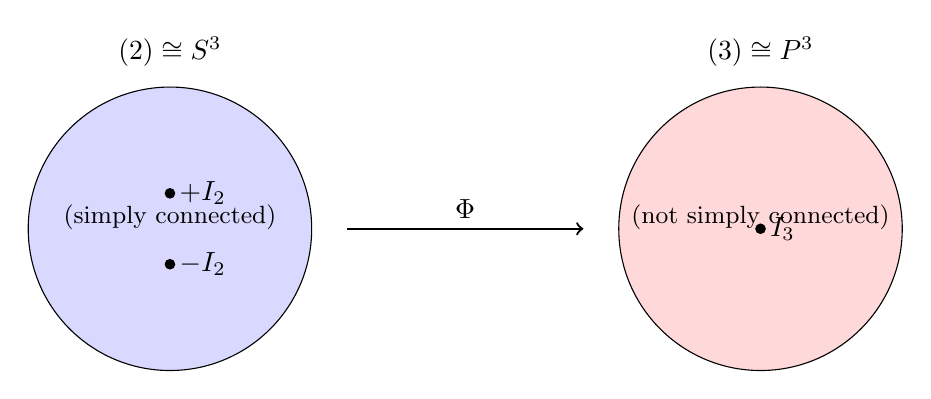
\begin{tikzpicture}[scale=1.5]
  % SU(2) as S^3
  \draw[fill=blue!15] (0,0) circle (1.2);
  \node at (0,1.5) {$\SU(2)\cong S^3$};
  \node at (0,0.1) {\small (simply connected)};
  \draw[fill=black] (0,0.3) circle (0.04) node[right] {$+\bm{I}_2$};
  \draw[fill=black] (0,-0.3) circle (0.04) node[right] {$-\bm{I}_2$};

  % Arrow
  \draw[->,thick] (1.5,0) -- (3.5,0) node[midway,above] {$\Phi$};

  % SO(3) as RP^3
  \draw[fill=red!15] (5,0) circle (1.2);
  \node at (5,1.5) {$\SO(3)\cong \R P^3$};
  \node at (5,0.1) {\small (not simply connected)};
  \draw[fill=black] (5,0) circle (0.04) node[right] {$\bm{I}_3$};
\end{tikzpicture}
\end{center}

\pause
\vspace{0.5em}
\textbf{Why two-to-one?}  Both $\bm{U}$ and $-\bm{U}$ give the same rotation.
A rotation by angle $\theta$ about axis $\hat{\bm{n}}$ lifts to
$\pm\cos(\theta/2)\bm{I}_2 \mp i\sin(\theta/2)(\hat{\bm{n}}\cdot\bm{\sigma})$.
Increasing $\theta$ by $2\pi$ flips the sign!
\end{frame}

% ======================================================================
\section{Lie Algebra Isomorphism \texorpdfstring{$\so(3)\cong\su(2)$}{so(3)≅su(2)}}

\begin{frame}{Lie Algebra Isomorphism \texorpdfstring{$\so(3)\cong\su(2)$}{so(3)≅su(2)}}
\begin{block}{Theorem}
Define $\phi:\so(3)\to\su(2)$ by $\phi(\bm{L}_i) = \bm{T}_i$
(and extend $\R$-linearly).  Then $\phi$ is a Lie algebra isomorphism.
\end{block}

\pause
\begin{block}{Proof (essence)}
\begin{itemize}
\item $\phi$ maps a basis to a basis $\implies$ linear isomorphism.
\item Both satisfy $[\bm{L}_i,\bm{L}_j]=\varepsilon_{ijk}\bm{L}_k$
and $[\bm{T}_i,\bm{T}_j]=\varepsilon_{ijk}\bm{T}_k$.
\item Therefore $\phi([\bm{L}_i,\bm{L}_j]) = \phi(\varepsilon_{ijk}\bm{L}_k)
= \varepsilon_{ijk}\bm{T}_k = [\bm{T}_i,\bm{T}_j] = [\phi(\bm{L}_i),\phi(\bm{L}_j)]$.
\end{itemize}
\end{block}

\pause
\vspace{0.5em}
\textbf{Significance:} Although $\SU(2)$ and $\SO(3)$ are different as groups
(double cover vs.\ quotient), their Lie algebras are \textbf{identical}.
Infinitesimal rotations are the same in both pictures.
\end{frame}

% ======================================================================
\section{Summary and Next Steps}

\begin{frame}{What We've Built So Far}
\begin{enumerate}
\item \textbf{Topological spaces} $\to$ \textbf{topological manifolds}
$\to$ \textbf{smooth manifolds} — the geometric foundation.

\pause
\item \textbf{Groups, fields, vector spaces, Lie algebras} — the
algebraic foundation.

\pause
\item \textbf{Lie groups} = smooth manifolds + groups —
where geometry meets algebra.

\pause
\item Every Lie group has a \textbf{Lie algebra} (tangent space at identity
with commutator bracket).

\pause
\item The \textbf{Closed Subgroup Theorem} lets us recognize matrix Lie
groups easily.

\pause
\item $\SO(3)$ (rotations) and $\SU(2)$ (unitary $2\times 2$ matrices)
are the central examples.

\pause
\item $\SU(2)$ is a \textbf{double cover} of $\SO(3)$.
Their Lie algebras are \textbf{isomorphic}: $\so(3)\cong\su(2)$.
\end{enumerate}
\end{frame}

\begin{frame}{What Comes Next (Part II)}
\begin{block}{Representation Theory (next meeting)}
\begin{itemize}
\item Representations of Lie algebras and Lie groups.
\item Complexification $\su(2)_\C \cong \mathfrak{sl}(2,\C)$
and the Cartan--Weyl basis $(\bm{H},\bm{E},\bm{F})$.
\item Classification of irreducible representations of $\su(2)$:
for each $j\in\{0,\tfrac12,1,\tfrac32,\dots\}$,
a unique irrep of dimension $2j+1$.
\item Integration: every $\su(2)$-representation exponentiates
to an $\SU(2)$-representation.
\item Projective representations and the descent to $\SO(3)$:
integer $j$ $\to$ ordinary representations,
half-integer $j$ $\to$ spinor (projective) representations.
\item Physical spin operators and the $4\pi$ periodicity of spinors.
\end{itemize}
\end{block}
\end{frame}

\begin{frame}{References}
\begin{itemize}
\item Hall, B. C. (2015). \textit{Lie Groups, Lie Algebras, and
Representations: An Elementary Introduction} (2nd ed.). Springer.

\item Lee, J. M. (2012). \textit{Introduction to Smooth Manifolds}
(2nd ed.). Springer.

\item Steinacker, H. (2024). \textit{Lie Groups and Lie Algebras
for Physicists}. Lecture notes, University of Vienna.

\item Full paper with proofs:
\href{https://raw.githubusercontent.com/ganddoffcha/quantum-spin/main/gordon-chan-quantum-spin.pdf}
{\texttt{github.com/ganddoffcha/quantum-spin}}
\end{itemize}
\end{frame}

\begin{frame}
\begin{center}
\Huge Thank you!\\[1em]
\Large Questions?
\end{center}
\end{frame}

\end{document}
